\documentclass[conference]{IEEEtran}

\ifCLASSINFOpdf
   \usepackage[pdftex]{graphicx}
   \graphicspath{{../pdf/}{../jpeg/}}
   \DeclareGraphicsExtensions{.pdf,.jpeg,.png}
\else
\fi

% correct bad hyphenation here
\hyphenation{op-tical net-works semi-conduc-tor}

% CUSTOM PACKAGES
\usepackage{amsmath}
\renewcommand{\arraystretch}{1.3}
\usepackage{etoolbox}
\apptocmd{\thebibliography}{\setlength{\itemsep}{3pt}}{}{}
\usepackage{url}
\usepackage{caption}
\usepackage{subcaption}
\usepackage{colortbl}
\usepackage{xcolor}
\definecolor{light-gray}{gray}{0.78}
\usepackage{epstopdf}
\usepackage{lettrine}
\usepackage{listings}


\begin{document}
\lstset{
  frame=none,
  xleftmargin=2pt,
  stepnumber=1,
  numbers=left,
  numbersep=5pt,
  numberstyle=\ttfamily\tiny\color[gray]{0.3},
  belowcaptionskip=\bigskipamount,
  captionpos=b,
  escapeinside={*'}{'*},
  language=haskell,
  tabsize=2,
  emphstyle={\bf},
  commentstyle=\it,
  stringstyle=\mdseries\rmfamily,
  showspaces=false,
  keywordstyle=\bfseries\rmfamily,
  columns=flexible,
  basicstyle=\small\sffamily,
  showstringspaces=false,
  morecomment=[l]\%,
}


\title{Farfalle: a Domain-Specific Language for Processor Instruction Sets}

\author{
\IEEEauthorblockN{Alessandro de Gennaro}
\IEEEauthorblockA{School of Electrical and\\Electronic Engineering\\
Newcastle University\\
Newcastle upon Tyne, United Kingdom\\
Email: a.de-gennaro@ncl.ac.uk}
\and
\IEEEauthorblockN{Paulius Stankaitis}
\IEEEauthorblockA{School of Computing Science\\
Newcastle University\\
Newcastle upon Tyne, United Kingdom\\
Email: paulius.stankaitis@ncl.ac.uk}
\and
\IEEEauthorblockN{Andrey Mokhov}
\IEEEauthorblockA{School of Electrical and\\Electronic Engineering\\
Newcastle University\\
Newcastle upon Tyne, United Kingdom\\
Email: andrey.mokhov@ncl.ac.uk}}

\maketitle

\begin{abstract}
Adopting a systematic approach for the design of processor instruction sets is
instrumental for tackling the complexity of modern processors.

We present a tool-chain which follows the designer through all the design phases,
from the specification of instructions to the hardware synthesis of a
microcontroller. The flow is also meant to facilitate the understanding of the
Instruction Set Architecture (ISA) reference manuals. Often, these documents are
semi-formal, hard to read and fully understand, especially when dealing with
highly concurrent implementations. We believe that designers will also
benefit from a visual graph-based model, automatically derived from the ISA
specification, and customisable to fit different needs. Some of the tools have
already been developed and tested on ARMv6-M architecture, others yet need to be
fully implemented. The design flow will be integrated into the Workcraft framework.

This paper presents a new domain-specific language for ISA specification and demonstrates
how it can be used for the specification of ARMv6-M microcontroller. We also compare
the presented approach with the others available in the literature.
\end{abstract}

\IEEEpeerreviewmaketitle

\section{Introduction}
\label{sec:intro}
Technology progress allows industries to integrate always more transistors over the
same amount of area, following Moore's law. In turn, design complexity of these
systems progressively increases. This led research to be focused on raising the
level of abstraction of the languages used at the early-stages of design. This work
presents a design flow for an easier specification, visualisation, simulation,
customisation and hardware synthesis of instruction sets.

The consultation of an ISA reference manual (i.e. ARMv6-M~\cite{armManual}) can be
difficult and tedious. Anthony Fox, in his attempt to describe a model
of the ARMv7 instruction set, argues: ``official reference manuals are large,
stretching to many hundreds of pages - one can easily overlook subtle details or
become bogged down with ``uninteresting'' background information''~(\cite{armv7},
Section 1). And yet: ``official descriptions are semi-formal (ambiguous)''~(\cite{armv7}, Section 1). 

In the light of the above, a simple and formal way to specify and, more
specifically, visualise instruction sets is needed. A visual graph-based model can
help designers for a quicker comprehension of the processor. ISAs in fact provide a
software level description of the hardware itself. We use Conditional Partial Order
Graph (CPOG)~\cite{cpog}\cite{andreyPhd} as the visualisation model. They can
efficiently represent concurrent and sequential behaviours, and already come with a
tested tool-kit for the customisation, encoding and hardware synthesis~\cite{workcraft}\cite{satEncoding}\cite{acsd}.

We propose a new domain-specific language for ISA specification. The current
implementation is embedded in \textit{Haskell}~\cite{haskell}. This is a high-level
functional language that provides static type checking and inference capabilites,
as well as useful predefined constructs and classes that we rely on in our
implementation (i.e. the Monad class).

The article is organised as follows: Section~\ref{sec:dsl} describes the framework
we have developed, and how this can be used to interact with all the steps of the 
design flow. Section~\ref{sec:arm} presents a case-study: the ARMv6-M ISA and how it
can be converted into a more comprehensible CPOG representation. 
And finally, Section~\ref{sec:conclusion} summarises the achieved results, 
outlining the future research directions.

\subsection{Related work}

An attempt to use partial orders to describe the instructions of a complex hardware
structure can be found in~\cite{maxPhd}. The author uses Conditional Partial Order
Graphs to visually describe the instructions of the Intel 8051 Microcontroller.
Yet, he used them for building an asynchronous controller and managing the internal
execution flow of the datapath elements. The manual construction of partial orders
is an error-prone process. Connecting all the operations, taking into account their
dependencies and order, is a complex task. This further inspired our research, and
led us to bridge this gap with an automated approach.

Regarding the language we chose to adopt, it is not difficult to find other cases
where functional languages have been used as a starting point for ISA
specification. In this direction, \cite{isaFunc} provides an interesting attempt to
build an infrastructure for instruction set development. The authors developed the
concepts of \textit{state} and \textit{transformations}. The former represents the
current state of the machine, which evolves over time according to the
transformations (instructions). \textit{F. Yuan and K. I. Eder} instead, created a
formal and hierarchical model, which can be refined for fitting the needs of a
particular ISA. This model (characterised in \cite{isaEventB}) is composed by 4
abstract layers. Each of these layers describes a particular aspect of the
instruction set. The deeper the designer explores this hierarchical representation,
the more refined will be the final system.

Another example can be found in \cite{armv7}. The authors, in there, built a framework
which can be extended to tailor instruction sets. They use the monadic programming
style, based on three basic operations: \textit{return}, \textit{bind} and
\textit{parallel}. These are meant to mimic the flow of an entity (the hardware
system), which is always returned as a result of the execution of an instruction.
Instructions can be bound together either sequentially or in parallel. Here, the
case study used is the ARMv7, a widespread instruction set embedded by the 
Cortex-A8 processor. An additional example of how an ISA might be specified inside
a tool is present in \cite{isaXml}. Both the modules and the instructions here are
introduced via a xml-based language, fairly readable but not very flexible.

In this work we aim at developing a domain-specific language based on Haskell. This will be
adopted for the representation of the ARMv6-M, used as the case study. The target
representation abstracts some details such as the bit-length of the registers or immediate
values. The goal is the integration of the framework presented in Section~\ref{sec:struct}
into a systematic design flow (Section~\ref{sec:func}), and the simplification of the understanding of
processor instruction sets with a graph-based model (Section~\ref{sec:read}).

%------------------------------------------------

\section{A Domain-Specific Language: Farfalle}
\label{sec:dsl}
The language used to describe the framework is Haskell~\cite{haskell}. This is a 
functional language with high abstraction capabilities.
We followed the path, already explored in \cite{armv7}, implementing the \textit{monad class}
to build the infrastructure of the domain-specific language (DSL).

In Farfalle, the processor is seen as an entity composed by a combination of an internal and
external storage. Respectively, the former is represented by a set of registers,
while the latter by a memory that contains both instructions and data; in compliance with the
von Neumann architecture. 

The processor executes instructions, that modify the state of the modelled machine.

$$P(Regs, Mem) \Rightarrow P'(Regs, Mem)$$

\noindent Every time the processor executes an instruction indeed, the state of the system
evolves into a new state $P'$ different from the previous one. Where either the registers and
the memory might be different. This approach is relatively similar to the processor
description in \cite{isaFunc}. Therefore, we are confident that the high degree of
abstraction obtained will allow the bidirectional connection of these two representations.

This section is organised as follow: Section~\ref{sec:struct} describes the structure of the
framework. A characterisation of the design flow derived by this approach is presented in
Section~\ref{sec:func}, while a brief description of the verification side, related to Event-B
interpretation, is discussed in Section~\ref{sec:ver}.

\subsection{Structure of the framework}
\label{sec:struct}
What marks our approach is the high degree of flexibility and abstraction that can
tailor to every processor. The framework we present in this document is composed
by different layers (modelled in various and interconnected modules). Each of them plays 
an important role in the structure.

The module in charge of modelling the low-level hardware functions is named
\textit{basics}. Positioned at very bottom layer, defines the ways through which the
memory elements can be accessed, the behaviour of the data-path components, 
as well as the monad basic functions: return and bind.

Furthermore, the types used in the structure are defined.
The registers and the memory are internally implemented with two maps of integer values.
The former can be accessed either via the name of a
special purpose register, or using the pattern $R \; Int$ (i.e. $R \; 5$, to point out the
fifth location in the register file). Memory is accessed via an integer type address instead.
Immediate values are also internally seen as integers. This approach is not
accurate. Some of the features -- the bit length of the registers, or the
endianness of the data -- are lost. Nonetheless, the high level of abstraction of
the framework allows the interpretation of the model from several points of view (see
Section~\ref{sec:func}), and is eventually enough for the control unit synthesis.

Finally, ComputationType is defined. This is a flexible type in input to the
arithmetic logic unit (ALU), which can be modified according to the ISA
needs. As far as this unit is concerned in fact, different combinations of inputs can be
given to it: one single register for an increment/decrement operation, either two 
registers, or one register and an immediate for an ADD/SUB/MUL operation, and so on.
Therefore, ComputationType is not a fixed type and can be extended for fitting different
ALU architectures.

\textit{Microprogram} is the interface based on the low-level module just described.
In this, just a few operations, generically present in a general purpose processor, are
implemented. The function for incrementing the program counter and fetching
the next instruction, the pop and push instructions, the interface methods for accessing
the registers and memory (internally modelled in the module basics).
In addition to the set of internal registers usually contained in a generic processor,
this module defines three registers more: the program counter, the instruction register and
the stack pointer.

\textit{ISA\_model} is the module where the user is supposed to introduce the custom 
instruction set architecture. Based on the bottom layers, this
module can be customised adding other special purpose registers and extending ALU types.
Most importantly, this will contain all the instructions one wants to include in a custom ISA.
This will act as an interface for the software-level simulation and will be taken into
account for the conversion towards other models and languages (Section~\ref{sec:func}).

\textit{Main} is the module meant for the high-level software simulation, in here
all the instructions can be executed over the processor modelled. This might be useful
for having a first proof of a consistent architecture. Indeed, the possible implementation
errors can be captured analysing the behaviour of the whole system.

\begin{figure}[ht!]
\begin{center}
	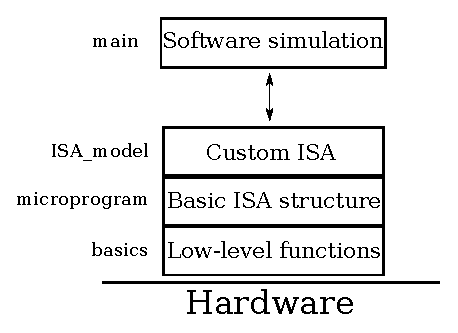
\includegraphics[scale=1]{IMG/structure.eps}
	\caption{Functional structure of the framework.}
	\label{fig:structure}
\end{center}
\end{figure}

In Figure~\ref{fig:structure}, the structure of the framework is depicted, pinpointing 
on the interconnections between the modules described. The structure is rather simple
and small, and can be potentially extended with new procedures and types, making
this approach flexible and scalable.

In Section~\ref{sec:arm} we will show how this framework has been implemented and extended
to model the ARMv6-M.

\subsection{Functionalities \& interpretations}
\label{sec:func}
Our main goal with this article is to open the path towards an easier specification and
visualisation of instruction sets. Nonetheless, quite a few other interpretations can be
given to this work. The domain-specific language indeed, once used to model
a processor, can be potentially translated into other languages. In turn, they
can be progressively employed with the advantages and tools they come with. It is worth
mentioning that some of the functionalities discussed in this section have not been
implemented yet. Though, they will be part of our future work (see Section~\ref{sec:frd}).

The ISA specification might be converted into Event-B language~\cite{eventB}. This is a
formal technique used to analyse the model at the system level. It comes with some theorem
provers which are able to verify the consistency of the system, proving that there are 
no inconsistencies between instructions. This is an interesting feature itself, which could
be particularly useful when applied to instruction sets. It falls within the side of the
formal \textit{verification} (see Section~\ref{sec:ver} for a detailed description).

\textit{Visualisation} and \textit{synthesis} are two other
interpretations which can be given to this framework, connected to each other via the
CPOG formalism. Even though Haskell provides readable and simple constructs, instruction
set specifications are intrinsically difficult to read and understand.
Capturing all the dependencies between the micro-operations within instructions is
complex and error-prone. Reading the whole reference manual can take a long time.
In the light of the above, formal specification can be converted into partial orders,
a visual graph-based representation composed by nodes and arcs, much more comprehensible 
than reference psuedo-code or Haskell statements.

\begin{figure}[ht!]
\begin{center}
	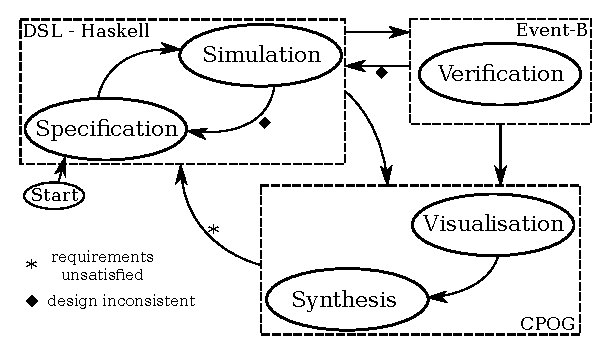
\includegraphics[width=\linewidth]{IMG/flow.eps}
	\caption{Design flow supported by Farfalle.}
	\label{fig:flow}
\end{center}
\end{figure}

This allows the user to employ the tool-chain around the conditional partial order
graphs, enabling the visual customisation of the dependencies of the instructions in 
\verb|Workcraft| and CPOG-based synthesis tools. A fairly
accurate measurement of the size of the final microcontroller for the processor control
unit can be automatically derived therefore, allowing the designer to come back at the
specification phase if some of the requirements (area, power consumption) have not been
met.

The whole design-flow is illustrated in Figure~\ref{fig:flow}.

\subsection{Verification with Event-B}
\label{sec:ver}
Design validation process is instrumental for any kind of systems. A typical system design
process requires numerous minor optimization modifications. The system needs to be 
re-validated after each refinement step, making this phase not particularly cost and time
effective. Applying formal techniques is a complex task, which requires a deep mathematical
understanding and rigorous analysis of the system. Furthermore, training domain specific
engineers to mathematical techniques can be very expensive. Therefore, our approach will
include methods and tool support, which intends to hide mathematical complexity by automating
validation process. 

Event-B~\cite{eventbbook}, originated from well known formalism called B method, is one of the most used
specification languages in safety critical software development area. Over the years, Event-B
proved to be successful mainly due to a few large academic research projects. Nowadays, this
is commonly used in industry. Excellent tool support and proof driven process~\cite{summevent} 
were key aspects which led us to choose this particular method.

The formalism is based on First Order Logic and Zermelo-Fraenkel set theory. This is a
high-level and expressive language. System specification is the initial
step in formal validation and it starts with describing requirements for the design. System
requirements should completely cover functionality and environment of the design. Next stage
is represented by the system development. Here, the model is developed: starting with the most
abstract model, this is gradually refined broadening the level of granularity.

Formal verification is another major branch of formal modelling. After the system is
specified and abstracted, its conditions need to be rigorously proved. Model is considered
correct if and only if all conditions, also known as \textit{proof obligations}, are
satisfied. Beforehand, designer is required to define invariants of the system, which need to
hold as system progress. In Event-B these conditions are used to construct verification
conditions for Invariant Preservation Rule. There are few of these rules, but the most
important are Invariant Preservation Rule, Deadlock Freedom Rule and also satisfaction of
refinement obligation. These set of rules just indicates what needs to be proven.

\begin{figure}[ht!]
\begin{center}
	$$\begin{cases}
	A(c)\\
	I(c, v) & \vdash \quad I_i(c, E(c,v))\\
	G(c, v)
  \end{cases}$$
	\caption{Invariant Preservation Rule}
	\label{fig:eveB}
\end{center}
\end{figure}

In Figure~\ref{fig:eveB}, sequent of Invariant Preservation Rule is stated, where hypothesis
consists of axioms, invariants and guards of the events. The goal is to validate whether
invariants hold after event.

%------------------------------------------------

\section{A case study: ARMv6-M}
\label{sec:arm}
Case study section intends to demonstrate potential of our domain specific language by
analysing ARM Cortex M0+ microprocessor instruction set. This section starts with a brief
description of the ARMv6-M instruction set and information we used to construct our model
(Section~\ref{sec:feat}). Further, concrete example of translated instruction to is
demonstrated together with visual graph representation (Sections~\ref{sec:mod} and
\ref{sec:read}). As the basis for our experiment, we used microprocessor
manual~\cite{armManual}, which includes short descriptions of each instruction as well as
functionality pseudocode and encodings. We used this information to build an instruction set
model of this specific microprocessor. 

\subsection{Features \& issues at the specification phase}
\label{sec:feat}
The faithfulness of ARMv6-M model with the reference specification was our main concern.
We aimed at representing each instruction listed in the ISA document using the
framework presented in this work, with the least loss of information. This required to be
as consistent as possible with the manual, replicating the flow of the operations with
the same order, as well as using the same names of the variables and functions at times.

As far as the reference documents are concerned, instructions characterised in there tend to
come up with a bare description. Hence, sometimes being completely accurate with 
the source system is complex, also because of the lack of technical information about the
original architecture. This was the case for some of the functions such as DataMemoryBarrier,
BkptInstrDebugEvent, Hint\_SendEvent, and so on~\cite{armManual}.
None of them are described in the reference manual, therefore these
functions are considered to be executed atomically (by one single node). Obviously, this
might not be the case and a deeper research with the producers of the core is needed to
untangle these operations.

Based on the structure described in Section~\ref{sec:struct}, we built the model on top of
the microprogram module. Therefore, many of the instructions characterised are supported by
the methods present at the bottom layers. For instance, the operation
\textit{incAndFetchInstruction} (depicted in the partial order in Figure~\ref{fig:andPO})
consists of three sequential micro-operations: incrementing the program counter (PC)
register, writing the result back into such a register and eventually moving the content of
the memory location pointed out by the PC into the instruction register (IR). This operation is
executed at the end of nearly all the instructions, except for the ones involving any branching
mechanisms. Another example which can be analysed is the \textit{pop} operation. It is in charge of
decrementing/incrementing the stack pointer (SP) register (according to the internal
architecture), and then fetching from the memory location addressed by the SP a chunk of 
data. These two operations are used inside the main instruction set architecture.

Another part which is worth discussing is the one related to the variety of the
registers present inside the core. Each of them has got a different function which we have
attempted to replicate as much as we could. In this case, the purpose of each register
is not described with much detail in the document. This partially limited the accuracy of the
final model. Nonetheless, the high degree of abstraction we kept downsizes the importance of
these problems. The registers present in our model are: linked register (LR), application
program status register (APSR), interrupt program status register (IPSR), execution program
status register (EPSR), the special-purpose mask register (also called PRIMASK), the 
special-purpose control register (CONTROL). They are needed to manage different internal
functions. In our model, we limited at reading and writing them according to the reference
description.

Additionally, all the arithmetic, logical and bitwise operations are represented in our
model. The lack of technical details is present also in this side, limiting the accuracy of
the model. We assumed that all these operations are
performed via the arithmetic logic unit (ALU). Unfortunately, this is just an
assumption, we are not sure whether the shift operation is truly accomplished
through such a unit or via another dedicated one, for instance.
This problem does not interfere with our main purpose of
developing a systematic approach though. Indeed, the designer of a system is expected to have
such a technical knowledge, which can be employed to reach a high degree of faithfulness in
the target model.

Given this general introduction about the model, in the next section some of the instructions
characterised in our representation will be showed, pinpointing at the high level of
similarity with the instruction set that we aimed at shaping.

\subsection{Target model description}
\label{sec:mod}
All the instructions included in the ARMv6-M have been characterised in our representation.
According to the reference manual description, the ARMv6-M is a subset of ARMv7-M and
supports Thumb 16-bit instruction set, including a small number of 32-bit instructions
introduced to the architecture as part of the Thumb-2 technology in ARMv6T2. 

\begin{figure}[ht!]
\begin{center}
	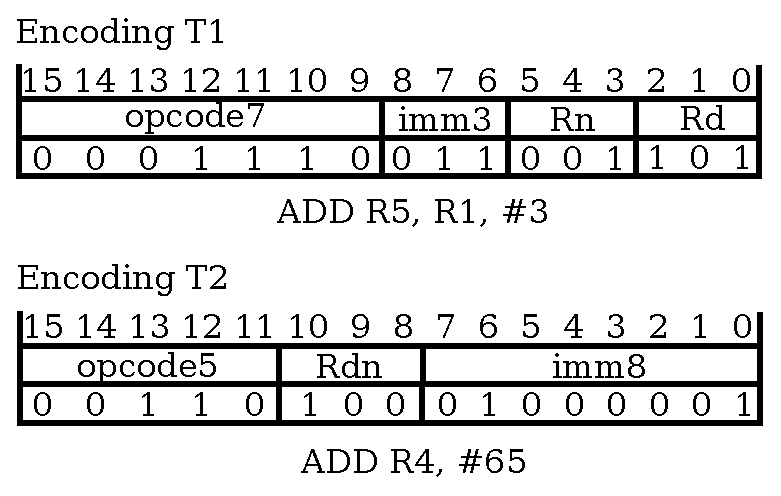
\includegraphics[width=8.2cm]{IMG/encodings_ex.eps}
	\caption{ADD (immediate) encodings - ARMv6-M~(\cite{armManual}, p.107-108)}
	\label{fig:ADDEnc}
\end{center}
\end{figure}

An interesting feature of the ISA is that some instructions have two opcodes, named T1 and
T2. This provides a more flexible architecture, which in turn comes up with a
flexible assembly language. This is the case for the \textit{ADD (immediate)} instruction,
for instance. The first encoding T1 has a seven bit opcode, and the rest of the
instruction encoding is meant for hosting an immediate value (3-bit), and two more register
locations (3-bit each): the source of the first operand and the destination of the result.
The second encoding \textit{T2} instead comes up with a quite different pattern. The opcode
associated to it is has only 5 bits, then there is a register (3-bit) which acts both as the
source operand and the destination of the result; the remaining 8 bits contain a longer
immediate value. Both of the encodings are depicted in Figure~\ref{fig:ADDEnc},
where also an example of how these two encoding might be used is present. These
instructions can be used for different purposes. Because of time constraints, we focused just
on the instructions with the encoding T1. Nonetheless, we plan to represent the
second encoding in future work, in order to create a fully realistic benchmark (see 
Section~\ref{sec:frd}).\\

\begin{lstlisting}[caption=ADD (immediate) instruction - Reference specification,
frame=single, label=lis:add]
EncodingSpecificOperations();
(result, carry, overflow) = AddWithCarry(R[n], imm32, '0');
R[d] = result;
if setflags then
    APSR.N = result<31>;
    APSR.Z = IsZeroBit(result);
    APSR.C = carry;
    APSR.V = overflow;
\end{lstlisting}

The pseudocode specification of the instructions have been translated into Farfalle 
(described in Section~\ref{sec:dsl}). During the conversion process, we
assumed that all the parameters which are involved in the internal operations are available
and ready to be used. This is the case for the \textit{imm32} value, for instance, present in
some of the instructions. This is over 32 bits, and is obtained extending the immediate value
present inside the instruction, over 3, 5 or 8-bit long at times. We assumed to have a
decoding function able to decode the instruction by the opcode. This is theoretically
supposed to execute the right operations (such as the immediate extension) prior to the
instruction execution.

Let us focus on the pseudocode specification of the ADD (immediate) instruction (showed in
Listing~\ref{lis:add}). Three parameters are needed for this instruction: \textit{R[n]},
\textit{R[d]} and imm32. \textit{setflags} is a flag always set to true for this instruction,
therefore is not considered in our implementation. We can similarly characterise this instruction
via the framework presented in this work, see Listing below.\\

\begin{lstlisting}[caption=ADD (immediate) instruction - Farfalle specification,
frame=single, label=lis:addH]
add_ImmT1 rn rd imm32 = do
    result <- alu (adcRegImm rn imm32 0)
    writeRegister rd result
    updateN result
    updateZ result
    updateC
    updateV
    incAndFetchInstruction
\end{lstlisting}

\noindent
The instructions takes in input two registers and an immediate value over 32 bits. According
to the reference document, the procedure \textit{EncodingSpecificOperation()} is the one in
charge of performing the right operations depending on the encoding read. As already
mentioned, we assume this step to be already performed beforehand to instruction execution.
All the other statements are quite similar to the source counterparts.
The only thing worth mentioning is that the alu operation is in charge of
setting the carry and the overflow bits internally. That is the reason why those two are not
present in the Haskell implementation. The \textit{IsZeroBit()} procedure simply checks if a
value is 0, this is implemented inside the function \textit{updateZ}. At the end of the
Haskell specification is present the \textit{incAndFetchInstruction}, which is in charge of
updating the program counter register and fetching the next instruction.

Another instruction which might be of interest is the store, also known as STR (register).
This instruction computes the address where to store a chunk of data, from a base
address and an offset, both defined into two registers. Although the offset can be optionally
shifted in a general ISA architecture, this feature has not been implemented in the ARMv6-M.
The \textit{shift\_n} variable in fact, which is supposed to contain the number of bits that
the register \textit{R[m]} must be shifted by, is always set to 0. Below the source
specification is showed:\\

\begin{lstlisting}[caption=STR (register) instruction - Reference specification,
frame=single, label=lis:str]
EncodingSpecificOperations();
offset = Shift(R[m], shift_t, shift_n, APSR.C);
address = R[n] + offset;
MemU[address,4] = R[t];
\end{lstlisting}

\noindent
The specification based on Farfalle is listed in Listing~\ref{lis:strH}.
According to the source description, this instruction takes in input three registers.
\textit{rn} contains the base address, \textit{rm} the optionally shifted offset (shifted by
0 bits in this implementation), and \textit{rt} that contains the data chunk to be stored
into the memory location pointed by the final result, eventually placed in the variable
\textit{address}. The arithmetic logic unit is in charge of performing either the shift and
the addition, as described in Section~\ref{sec:feat}. \textit{writeMemory} is one of the
procedure implemented in the module basics (see Section~\ref{sec:struct}). \textit{readBit}
procedure, simply returns the bit 29, where the carry flag is stored.\\

\begin{lstlisting}[caption=STR (register) instruction - Farfalle specification,
frame=single, label=lis:strH]
str_RegT1 rm rn rt = do
    offset <- alu (shlRegImm rm 0 (readBit apsr 29))
    address <- alu (adcRegImm rn offset 0)
    writeMemory address rt
    incAndFetchInstruction
\end{lstlisting}

The two Haskell-based specifications showed along this section are fairly similar to the
reference pseudocode. The degree of precision the designer can go for depends on the accuracy
the source specification have been characterised with. There has not been loss of
information in the conversion process.

\subsection{Visualisation}
\label{sec:read}
Going towards a more comprehensible ISA representation was one of our main goals. As discussed in
Section~\ref{sec:intro} in fact, often instruction set architecture reference documents are hard to
read and fully understand. We believe that having a visual representation of the operations
which occur inside each instruction would make the understanding easier and quicker. That is
the main reason why we chose to adopt partial orders to represent the behaviour of
instructions. Each instruction can be analysed singularly. The behaviour can be isolated,
focusing on the causality of the operations to execute.

\begin{figure}[ht!]
\begin{center}
	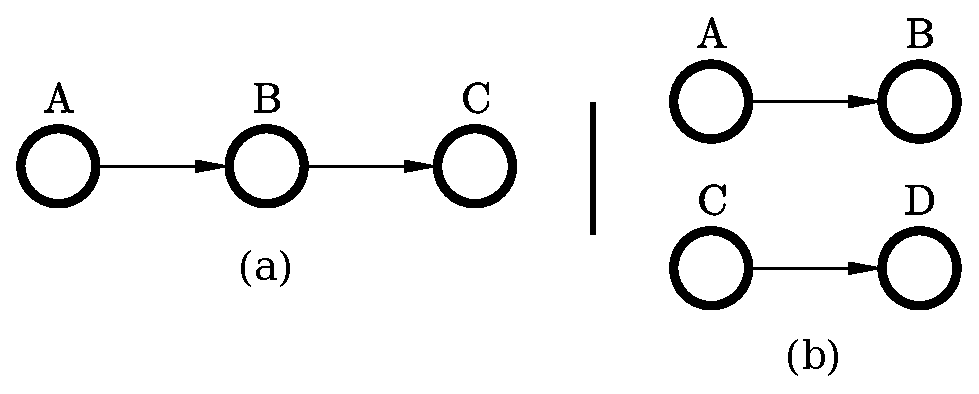
\includegraphics[scale=0.5]{IMG/pos.eps}
	\caption{Examples of sequential and concurrent behaviours.}
	\label{fig:pos}
\end{center}
\end{figure}

The capability of representing sequential and concurrent behaviours is instrumental for
modelling instructions. Partial orders address this requirement with the usage of nodes
($\bigcirc$) and dependencies ($\rightarrow$). Figure~\ref{fig:pos}(a) depicts a partial order
where the three operations are executed sequentially. Figure~\ref{fig:pos}(b) instead shows
four operations $\lbrace A,B,C,D \rbrace$ which can be executed with different orders. 
$A \rightarrow B$ and $C \rightarrow D$ are concurrent paths. A detailed
description can be found in \cite{andreyPhd}.

In the light of the above, we are working on automating the conversion process from the
Farfalle specification to partial orders. The tool will be able to analyse the
\textit{ISA\_module} file, capture the dependencies between the operations within each
instruction and build a partial order. 

Multiple levels of abstraction can be chosen for the conversion. Components such as the
arithmetic logic unit can be adopted for the execution of
different operations: i.e. addition, multiplication, shift, etc. One might want to represent
each single operation separately with a different node 
(trading off some readability with accuracy), or raise the
level of abstraction losing the internal information.

\begin{figure}[ht!]
\begin{center}
	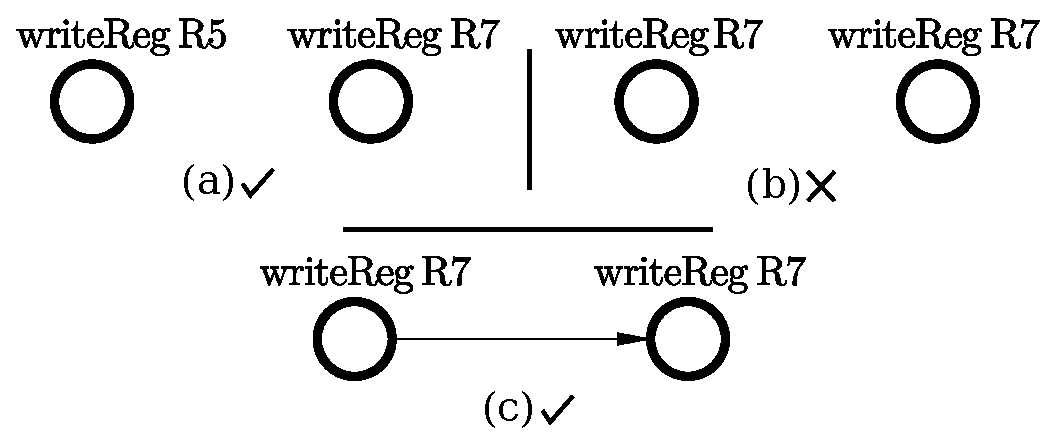
\includegraphics[width=\linewidth]{IMG/depPO.eps}
	\caption{Allowed and not allowed conversions.}
	\label{fig:depPO}
\end{center}
\end{figure}

The partial representation of the data, in some of the operations entailing registers and
memory access, represents another layer of abstraction which can be traded for readability.
This would allow the development of a more accurate model without overlapped register/memory
accesses. For instance, let us assume that the register file has got two different input
writing ports. This would allow two different registers to be written at the same time.
The destination of a writing operation should be taken into consideration therefore,
in order to avoid a simultaneous access at the same location of the register file
(see Figure~\ref{fig:depPO}). The partial order in Figure~\ref{fig:depPO}(b) is not allowed
because the two writing mechanisms can be triggered concurrently.
A dependency should be inserted, as in the graph in Figure~\ref{fig:depPO}(c).

The following example clarifies the above issue. 
Listing~\ref{lis:and} gives a specification of the AND (register) instruction (ARMv6-M ISA~\cite{armManual}).\\

\begin{lstlisting}[caption=AND (register) instruction - Farfalle specification,
frame=single, label=lis:and]
and_RegT1 rm rdn = do
    shifted <- alu (shlRegImm rm 0 apsr[29])
    result <- alu (andRegImm rdn shifted)
    writeRegister rdn result
    updateN result[31]
    updateZ result
    updateC carry
    incAndFetchInstruction
\end{lstlisting}

\noindent
This instruction can be automatically translated into the partial order in
Figure~\ref{fig:andPO}. Every statement of the specification corresponds to a node in the
graph. For instance, the one on fourth line correspond to the node named ``writeReg''.
The dependencies between the nodes are obtained by looking at the values which are needed for
the execution of each operation. For instance, the second ALU operation needs the value
called ``shifted'', computed during the first ALU operation. Therefore, the second action
depends on the first one.
``incAndFetchInstruction'' is a basic operation defined inside the module microprogram (see
Section~\ref{sec:struct}). This is composed by three sequential operations, which are in this
case extracted and depicted in the partial order, for an increased accuracy.

\begin{figure}[ht!]
\begin{center}
	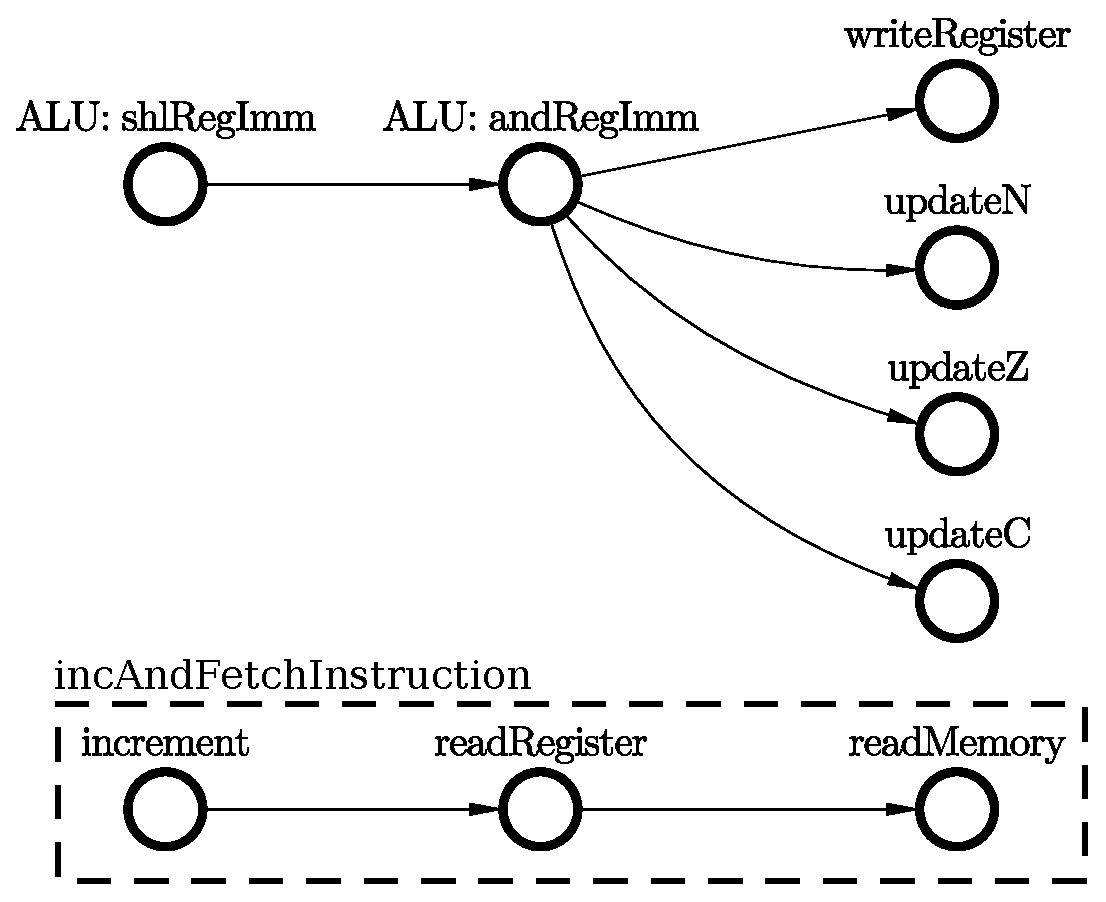
\includegraphics[width=\linewidth]{IMG/and_RegT1.eps}
	\caption{AND (register) instruction - ARMv6-M~(\cite{armManual},~p.116)}
	\label{fig:andPO}
\end{center}
\end{figure}

The graph in Figure~\ref{fig:andPO} is more readable than the Haskell-based specification,
listed in Listing~\ref{lis:and}. The dependencies between the various operations are
clearly expressed via arcs. In addition, the graph-based model provides a good degree
of fidelity; combined with the code-based specification it can lead to a good tradeoff
between readability and accuracy.

Another example which worths a discussion is the unconditional branch. This
instruction simply causes a branch to a target address. The Haskell-based specification is
depicted below:\\

\begin{lstlisting}[caption=B instruction - Farfalle specification,
frame=single, label=lis:and]
b imm32 = do
    nextInstrLocation <- alu (adcRegImm pc imm32 0)
    writeRegister pc nextInstrLocation
    readMemory nextInstrLocation ir
\end{lstlisting}

\noindent
The particularity of this instruction is the lack of the \textit{incAndFetchInstruction} step.
The new instruction register indeed is obtained by the address computed internally, adding an
32-bit immediate address with the current program counter register. In Figure~\ref{fig:bPO}
the partial order associate to the branch instruction is showed. The reader should notice that
there is no direct dependency between the \textit{writeReg} and the \textit{readMemory}
nodes. Nonetheless, a dependency has been inserted in order to fetch the new instruction once
that the PC register has been updated. This might be named a \textit{functional dependency}
and is implicit to the incAndFetchInstruction procedure either.

\begin{figure}[ht!]
\begin{center}
	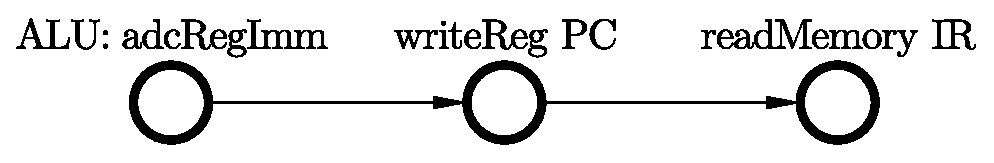
\includegraphics[width=8.7cm]{IMG/b.eps}
	\caption{Branch instruction - ARMv6-M~(\cite{armManual},~p.119)}
	\label{fig:bPO}
\end{center}
\end{figure}

We did not have the time yet to implement the tool for the conversion.
The example showed along this section has been obtained by hand. Therefore, we reserve for a
future article the results and considerations related to the synthesis of the final
controller.

\subsection{Instruction Verification}

This subsection briefly describes how instruction correctness can be validated. Constructing Event-B model
is refinement driven process, where developer starts with the most abstract concept of the system. We
started by declairing very basic concepts of microprocessors system. A typical, Event-B model structure
consists of context and machine frames, our intial context was used to declare some trivial constants and
data types e.g.  microprocessors' word size. Original context then was refined by adding more information
about operation type structure, decoding opcode/operands functions etc. For instance, in~(\ref{eq1}),
we state that instruction is pair type with opcode and three operands, whereas i.e. opcode-decode function
can be defined as shown in~(\ref{eq2}).

\begin{equation}
(opcode,(value, (value, value))) \in OPERATION
\label{eq1}
\end{equation}
\begin{equation}
DECODE \in OPERATION \rightarrow OPCODE
\label{eq2}
\end{equation}

After declaration of variables, types and structures in the context file, machine file was created, which
extended those concepts as well as included events. Machine model required further expansion of some key
concepts of data, registers, program counter, but most importantly it contained instruction events. In
Event-B, event can be conditional or unconditionally fired, depending on system requirements for that event.
In the context of the microprocessor and our model, event of the particular instruction is executed if
opcode satisfies the guard of the event. For example, (\ref{eq3}) shows one of the guards of the ADD
instruction.

\begin{equation}
DECODE(CODE(pc)) = ADD
\label{eq3}
\end{equation}

Satisfying guard condition means action in the event can be executed. In the context of ADD instruction
simple addition of two source registers is performed and the sum is loaded to the destination register,
which is then followed by increment of program counter register. 

However, analysis of ARM Cortex M0+ instruction set showed us that even simple instructions like addition
are difficult to specify formally in Event-B. Therefore, to make our model more feasible another refinement step would be
necessary in order to capture the same level of details as in specifications. Another important requirement
for instruction validation would be translation automation. Currently, we had to define the system and
correctness conditions as well as prove them. As stated before it is our objective to hide this mathematical
modelling exercise from engineers. Hence, together with creating a general framework, we need to automate
this process.

%------------------------------------------------

\section{Conclusion}
\label{sec:conclusion}
This work represents the first step towards a formal and readable specification of
processor instruction sets. We demonstrated how the specification of a real ISA, which has
been embedded into the \verb|ARM Cortex-M0|, can be specified via our framework without
loosing any information or lowering the accuracy of the representation.

In addition, we showed how such a framework can be converted into a visual-based
representation with different tradeoffs for maximising either the readability or the accuracy
of the graph-based model. The latter, based on the Conditional Partial Order Graph, can
exploit a built-in tool-chain embedded in \verb|Workcraft| for visualisation and hardware
synthesis purposes. In particular, this representation aims at simplifying the understanding of
the processor instruction sets.

This open-source framework~\cite{repo} opens the path towards different other languages and tools which
can be adopted in the design flow. Event-B might be one such piece of the puzzle which we
hope to be able to complete, together with the whole community in this field.

%Alex
\subsection{Future research directions}
\label{sec:frd}
Much research can be carried on about the work presented. First of all we will expand the
framework developed, providing some procedures to capture the internal instruction
dependencies, automatically deriving a partial order according to the level of abstraction
chosen by the user. This will be used to move from the DSL - Haskell framework, into the CPOG
representation (see Figure~\ref{fig:flow}), avoiding likely human errors. In turn, this will
allow us to derive the hardware microcontroller and make a consistent comparison (in terms of
area, power consumption, latency, etc.) with the one which the ARM Cortex-M0 embeds.

Secondly, we will work on a plugin to automatically convert the specification into the
Event-B language. This will allow the usage of sound theorem provers for the formal
verification of the ISA, an extremely useful instrument which designers might benefit from.

From the point of view of the case study itself, the model will be expanded to include the
T2 encodings. Other case studies will be carried out, such as the instruction
sets of the Texas Instruments MSP430 and the Intel 8051 processors. As is pointed out in
\cite{webArticle}, nowadays there are quite a few architectures with a relevant market size -
by ARM, ARC, Xtensa, MIPS. Unit volumes are progressively increasing, hence we believe the
need for modelling and experimenting by these companies will do so. Eventually, designers and
end users will benefit from a systematic approach to the design of processor instruction sets.

%------------------------------------------------

\begin{thebibliography}{10}

\bibitem{cpog}
	A. Mokhov, A. Yakovlev. \emph{``Conditional partial order graphs: Model,
	synthesis, and application''}. IEEE Transactions on Computers, Volume 59,
	Pages 1480-1493, November 2010.
	
\bibitem{andreyPhd}
	A. Mokhov. \emph{``Conditional Partial Order Graphs''}. Ph.D. Thesis,
	Newcastle University, September 2009.	

\bibitem{workcraft}
	I. Poliakov, D. Sokolov, A. Mokhov. \emph{``Workcraft: A static data flow
	structure editing, visualisation and analysis tool''}. Petri Nets and Other
	Models of Concurrency - ICATPN 2007. Pages 505-514, 2007.
	
\bibitem{satEncoding}
	A Mokhov, A Alekseyev, A Yakovlev. \emph{``Encoding of processor instruction
	sets with explicit concurrency control''}. Computers \& Digital Techniques,
	IET. Volume 5, Pages 427-439. November 2011.
	
\bibitem{acsd}
	A. de Gennaro, P. Stankaitis, A. Mokhov. \emph{``A Heuristic Algorithm for
	Deriving Compact Models of Processor Instruction Sets''}. 15th International
	Conference on Application of Concurrency to System Design (In Press). June
	24-26, 2015.

\bibitem{armv7}
	A. Fox, M. Myreen. \emph{``A Trustworthy Monadic Formalization of the ARMv7
	Instruction Set Architecture''}. Interactive Theorem Proving (ITP), pages
	243-258, 2010.	
	
\bibitem{isaEventB}
	F. Yuan, K. Eder. \emph{``A Generic Instruction Set Architecture Model in
	Event-B for Early Design Space Exploration''}. Technical Report CSTR-09-006,
	University of Bristol, September 2009.

\bibitem{isaFunc}
	T. A.Cook, E. Harcourt. \emph{``A Functional Specification Language for
	Instruction Set Architectures''}. Proceedings of the 1994 International
	Conference on Computer Languages. Publisher IEEE, pages 11-19. May 1994.
	
\bibitem{isaXml}
	A. Abbas, A. Ahmed, A. Ahmed, W. Uz Zaman Bajwa, A. Anwar, S. Abbasi. 
	\emph{``A retargetable tool-suite for the design of application specific
	instruction set processors using a machine description language''}. IEEE
	International Symposium on Circuits and Systems, 2002. Volume 1, pages 425-428.
	ISCAS 2002.
	
\bibitem{maxPhd}
	M. Rykunov. \emph{``Design of Asynchronous Microprocessor for Power
	Proportionality''}. Ph.D. Thesis, Newcastle University. Technical Report Series
	NCL-EEE-MICRO-TR-2013-182, December 2013.
	
\bibitem{armManual}
	ARM Ltd. \emph{``ARMv6-M Architecture Reference Manual''}. 
	ARM DDI 0419C (ID092410), 2010.
	
\bibitem{haskell}
	S. P. Jones (editor) et al.
	\emph{``Haskell 98 Language and Libraries The Revised Report''}.
	December 2002.
	
\bibitem{eventB}
	C. Métayer, J.-R. Abrial, L. Voisin. \emph{``Event-B Language''}. 
	Project IST-511599. $31^{st}$ May 2005
	
\bibitem{webArticle}
	J. Turley. \emph{``CPUs Get Cheaper; Transistors Get More Expensive''}. Electronic
	Engineering Journal: \url{http://www.eejournal.com/archives/articles/20151104-synopsys}.
	November 4, 2015
	
\bibitem{eventbbook}
    Abrial, Jean-Raymond. \emph{``Modeling in Event-B: System and Software Engineering''}.
    Cambridge University Press, New York, NY, USA.
    2010
    
\bibitem{summevent}
	J. Welte, H. Manz. \emph{``openETCS D2.1: Report on existing methodologies''}.
	ITEA2 Project Technical Report.
	January 2012
	
\bibitem{repo}
	A. Mokhov, A. de Gennaro, P. Stankaitis. \url{https://github.com/allegroCoder/microprograms}. Github repository.
    
\end{thebibliography}

\end{document}
